%
% teil3.tex -- Beispiel-File für Teil 4
%
% (c) 2020 Prof Dr Andreas Müller, Hochschule Rapperswil
%
% !TEX root = ../../buch.tex
% !TEX encoding = UTF-8
%
\section{Bestimmung durch drei Punkte
\label{moebius:section:teil4}}
\kopfrechts{Bestimmung durch drei Punkte}


Eine Möbius-Transformation kann eindeutig durch die Abbildung von drei Punkten bestimmt werden.

Gegeben seien drei Punkte \( A, B, C \) in der komplexen Ebene sowie drei zugehörige Bildpunkte \( A', B', C' \). Dann existiert genau eine Möbius-Transformation, welche die Punkte \( A, B, C \) auf die Punkte \( A', B', C' \) abbildet.

Für zwei Punkte existieren unendlich viele Möbius-Transformationen, die diese Bedingung erfüllen. Für vier Punkte ist das Gleichungssystem im Allgemeinen überbestimmt und besitzt keine Lösung.

Eine Möbius-Transformation besitzt zwar vier Parameter \( a, b, c, d \), jedoch nur drei Freiheitsgrade, da eine gemeinsame Skalierung dieser Parameter die Transformation nicht verändert.

\textbf{Beweis:}

Gegeben seien die Punkte:
\[
A = 0, \quad B = 1, \quad C = i
\]
und die Bildpunkte:
\[
A' = 1 + i, \quad B' = 0, \quad C' = i.
\]

Die Möbius-Transformation hat die Form:
\[
f(z) = \frac{az + b}{cz + d}.
\]

Wir bestimmen nun die Koeffizienten aus den Abbildungsbedingungen.

1. Bedingung:  \( A = 0 \mapsto A' = 1+i \)
\[
1+i = \frac{b}{d}
\quad \Rightarrow \quad
b = (1+i)d
\]

2. Bedingung:  \( B = 1 \mapsto B' = 0 \)
\[
0 = \frac{a + b}{c + d}
\quad \Rightarrow \quad
a + b = 0
\quad \Rightarrow \quad
a = -b = -(1+i)d
\]

3. Bedingung:  \( C = i \mapsto C' = i \)
\[
i = \frac{ai + b}{ci + d}
\]

Einsetzen von \( a \) und \( b \):
\[
i = \frac{-(1+i)di + (1+i)d}{ci + d}
\]

Faktorisieren von \( d \):
\[
i = \frac{d\left(-(1+i)i + (1+i)\right)}{ci + d}
\]

Zähler vereinfachen:
\[
-(1+i)i = -(i + i^2) = -(i - 1) = 1 - i
\]
\[
(1 - i) + (1 + i) = 2
\]

Damit:
\[
i = \frac{2d}{ci + d}
\]

Gleichung umformen:
\[
i(ci + d) = 2d
\]
\[
ic^2 + id = 2d
\]

Mit \( i^2 = -1 \):
\[
- c + id = 2d
\]

Trennung nach Real- und Imaginärteil:

Reell:
\[
- c = 2d \quad \Rightarrow \quad c = -2d
\]

Imaginär:
\[
id = 0 \quad \Rightarrow \quad d \neq 0 \text{ (Skalierungsfreiheit)}
\]

Parameterwahl:  \( d = 1 \)

\[
a = -(1+i), \quad b = 1+i, \quad c = -2, \quad d = 1
\]

Damit ergibt sich die Möbius-Transformation:
\[
f(z) = \frac{-(1+i)z + (1+i)}{-2z + 1}.
\]

Alternativ gekürzt:
\[
f(z) = \frac{(1+i)(1 - z)}{1 - 2z}.
\]

\textbf{Überprüfung:}

Wir betrachten die konkrete Darstellung:
\[
f(z)=\frac{(1+i)z + 1}{z + (1-i)}.
\]

Einsetzen der Punkte liefert:

\[
f(0)=\frac{1}{1-i}=1+i = A'
\]

\[
f(1)=\frac{(1+i)+1}{1+(1-i)}=\frac{2+i}{2-i}=0 = B'
\]

\[
f(i)=\frac{(1+i)i+1}{i+(1-i)}
=\frac{i+i^2+1}{1}
=\frac{i-1+1}{1}
=i = C'
\]

Damit wird gezeigt, dass die gewählte Möbius-Transformation die drei Punkte korrekt auf die gegebenen Bildpunkte abbildet.
Die drei Freiheitsgrade einer Möbius-Transformation entsprechen genau den drei frei wählbaren Punktabbildungen. Dadurch ist eine Möbius-Transformation durch drei Punktpaare eindeutig bestimmt.

\begin{figure}[h]
	\centering
	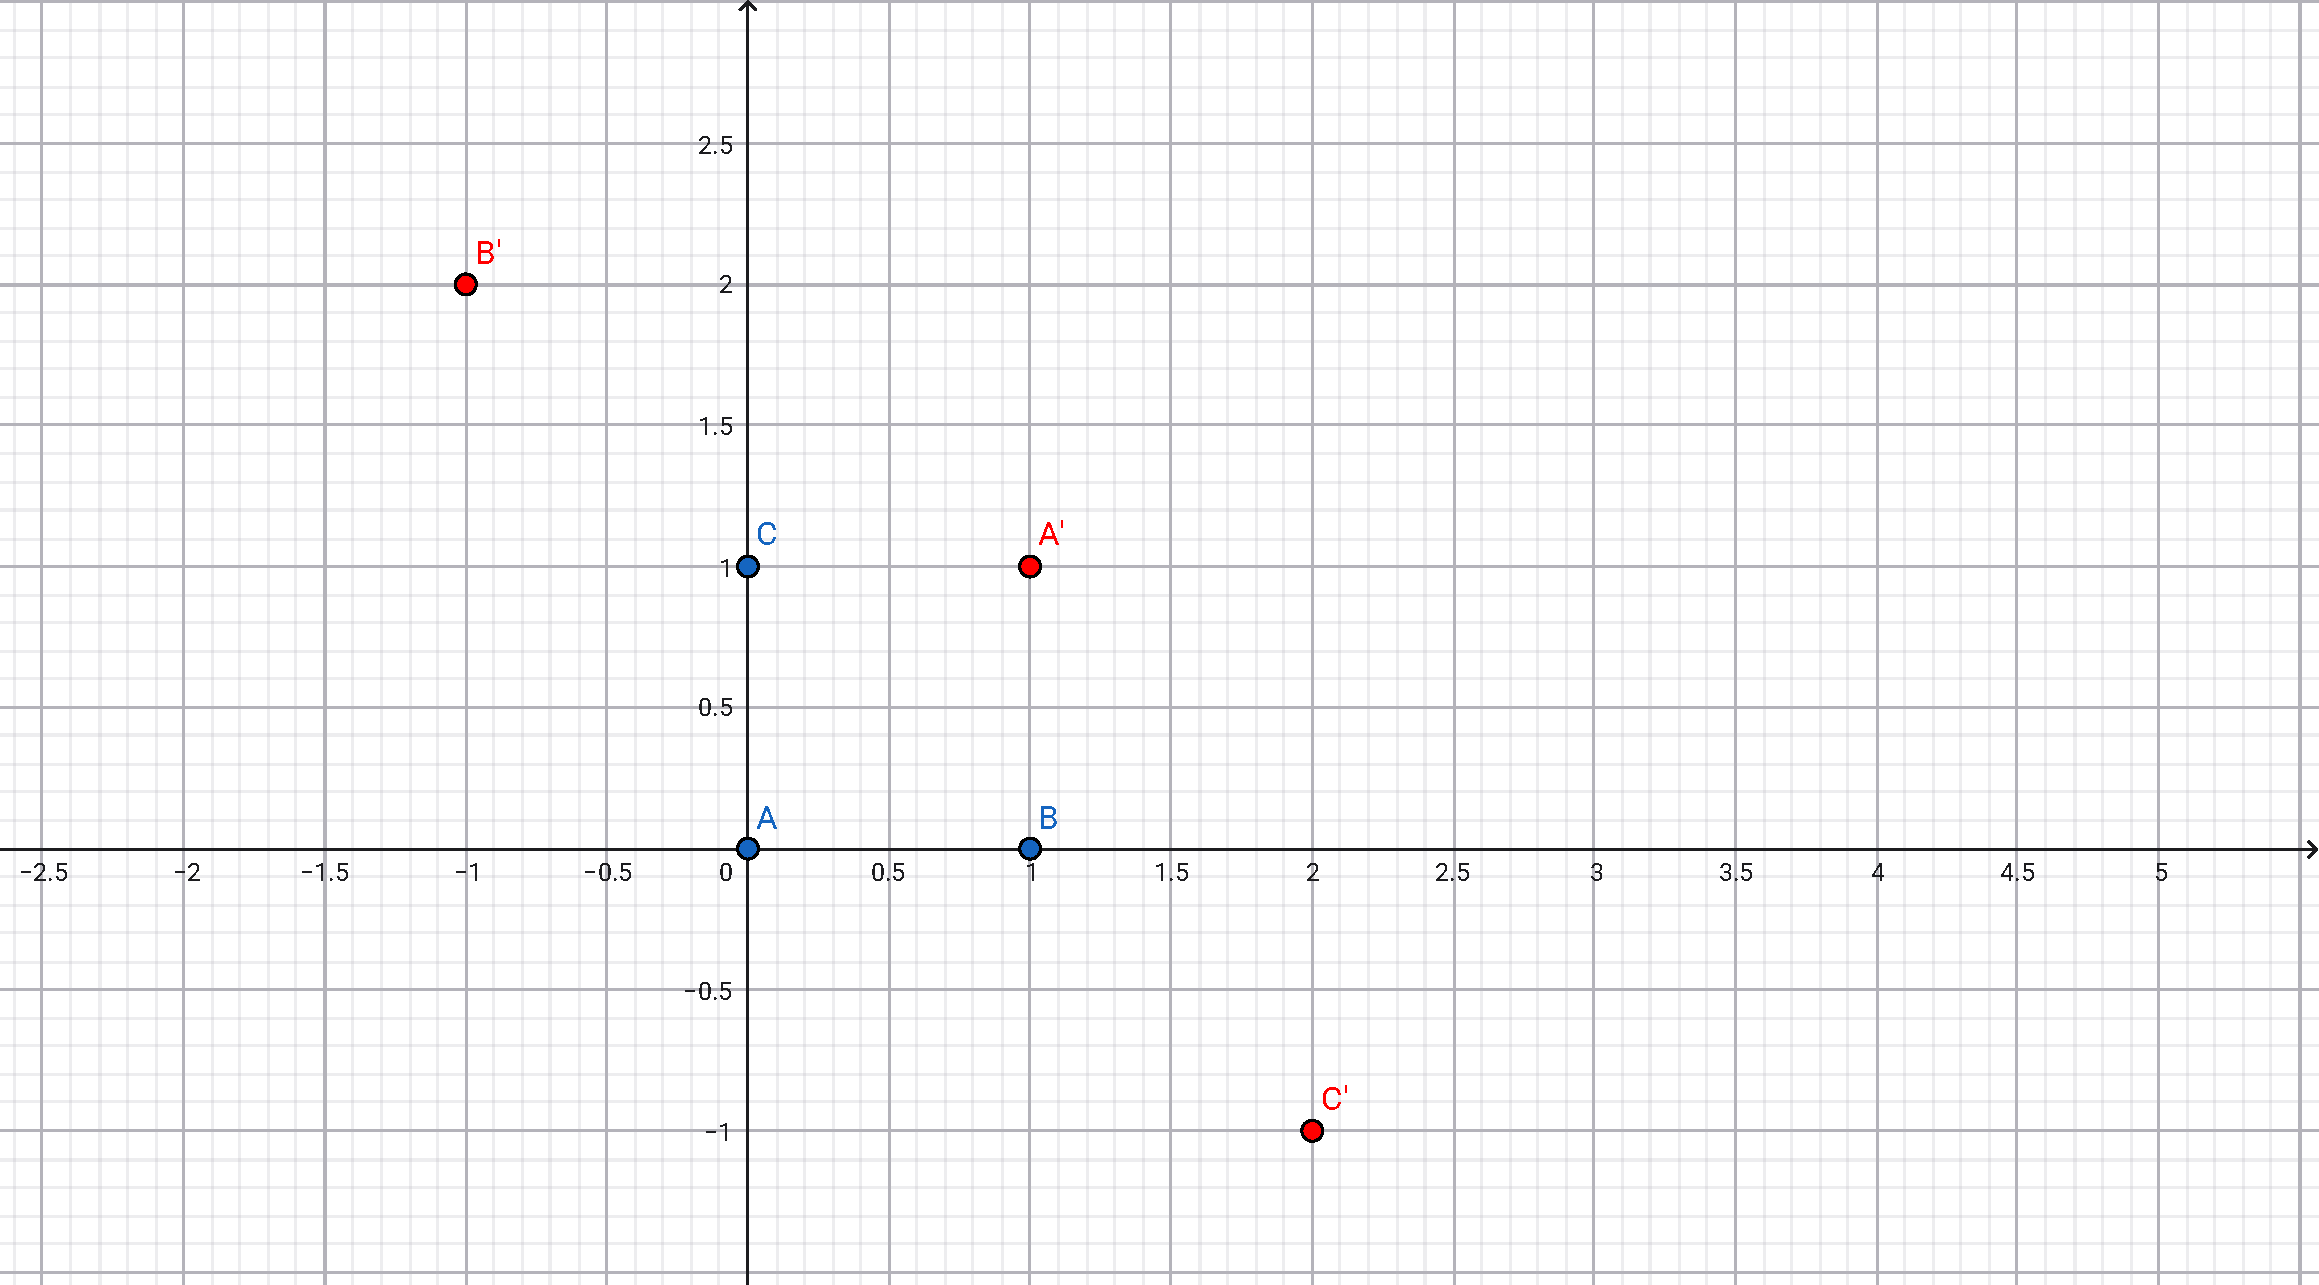
\includegraphics[width=0.6\textwidth]{bild7.pdf}
	\caption{Graphische Darstellung vom Beispiel oben}
\end{figure}